

\section{Network Disruptions}
\label{sec:interruption}

VCAs must handle network disruptions; they may do so in different ways.
Designing to cope with disruptions, such as interruptions to network
connectivity, has become even more pertinent over the past year as users have
increasingly relied on broadband Internet access to use VCAs, which can
sometimes experience connectivity disruptions.  In addition to experiencing
periodic outages, home networks are susceptible to disruptions caused by
temporary congestion along the end-to-end path.
In this section, we aim to understand how VCAs respond to the types of
disruptions that home Internet users might sometimes eperience. 


\subsection{Experiment Setup}

We analyze how
VCAs respond to temporary network disruptions during the call by introducing
transient capacity reductions. Using the same setup as in
Figure~\ref{fig:static_setup}, we initiate a five-minute VCA session between
two clients, C1 and C2, both of which are connected to the Internet via a
1~Gbps link. One minute after initiating the call, we reduce the capacity
between C1 and the router for 30 seconds, before reverting back to the
unconstrained 1~Gbps link. We repeat each experiment four times.
We conduct two sets of experiments: first disrupting the uplink, and then
disrupting the downlink. We reduce capacity to the following
levels: {0.25, 0.5, 0.75, 1.0} Mbps. (We do not consider disruptions in capacity
to levels of more than 1~Mbps because both Zoom and Meet's average utilization
is below 1~Mbps.)

\begin{figure}[t!]
\centering
\begin{subfigure}[t]{.5\textwidth}
    \centering
    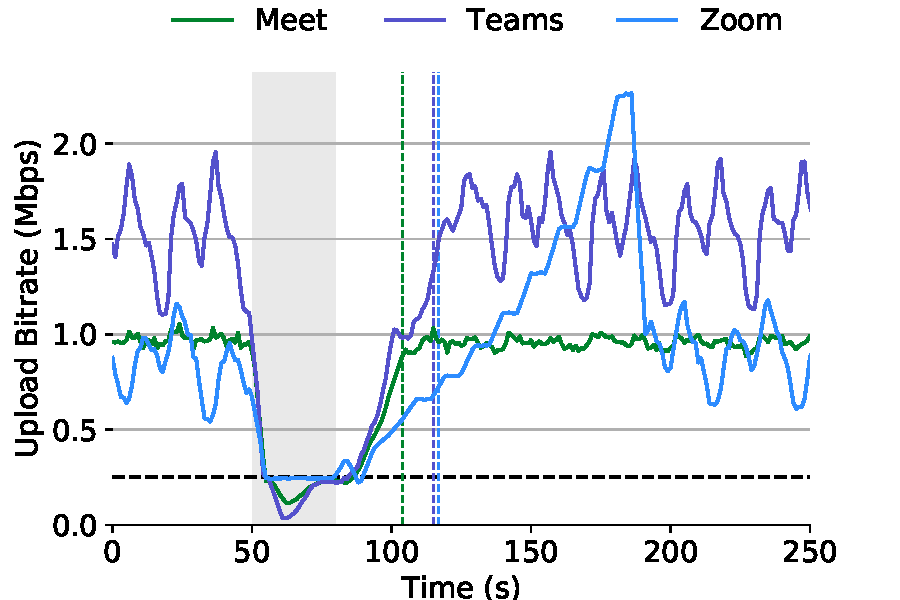
\includegraphics[width=.7\textwidth,keepaspectratio]{interrupt/Interrupt-upld.pdf}
    \caption{Average upstream bitrate over time. Grey region indicates period where uplink capacity is constrained to 0.25 Mbps. Vertical dotted lines indicate when the uplink bitrate has returned to the average.}
    \label{fig:ts_upld}
\end{subfigure}\hfill
\begin{subfigure}[t]{.5\textwidth}
      \centering
    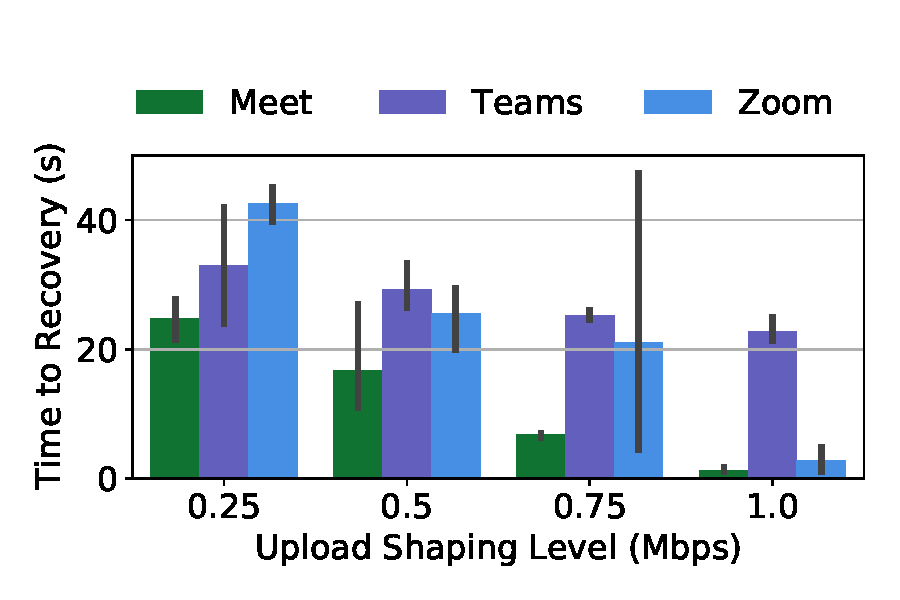
\includegraphics[width=.7\textwidth,keepaspectratio]{interrupt/TTR-upld.pdf}
    \caption{Time to recover.}
    \label{fig:TTR_upld}
\end{subfigure}
\caption{VCA response to a 30-second reduction in upstream capacity.}
\label{fig:interrupt-upld}
\end{figure}

\subsection{Upstream Disruptions}

Figure \ref{fig:ts_upld} shows VCA upstream bitrate over the course of a
call. Following a disruption, both the time to recovery and the
characteristics of that recovery
differ across VCAs. We quantify the time for
VCA utilization to return to normal by defining a 
\textit{time to recovery} (TTR) metric. We define TTR as the time between when the
interruption ends and when the five-second rolling median bitrate reaches the
median bitrate before interruption, also referred to as nominal bitrate. 

\paragraph{Time to Recovery}: Figure \ref{fig:TTR_upld} shows how extent of
the disruption to upstream connectivity affects each VCA's time to recovery.
The more severe the capacity reduction, the longer the VCAs need to recover.

\teams takes longer to recover even at less severe shaping levels for two
reasons: (1)~the nominal bitrate of Teams is higher than Meet and Teams,
(2)~Teams increases the upstream bitrate slowly immediately after the
interruption before increasing quickly back to normal (as shown in
Figure~\ref{fig:ts_upld}). Meet also observes a similar recovery pattern when
the disruption drops capacity to 0.25~Mbps. However, it recovers much faster
for the case of less severe disruptions, mostly because its nominal bitrate is
around 0.96 Mbps. 

\paragraph{Recovery Patterns}: While Meet and Teams follow a more rapid trend,
Zoom's recovery is different: It takes the longest time to recover under
severe disruptions. According to Figure \ref{fig:ts_upld}, Zoom follows a
stepwise recovery, with an almost-linear increase immediately after
interruption. It then enters into a periodic-probing phase where it increases
the sending rate, stays at it for sometime before increasing it again. The
probing phase continues well above the its nominal bitrate, before finally
reducing the bitrate.  Zoom does not return to a steady-state sending pattern
until two minutes after the disruption, in the meantime sending at much higher
rates. At first glance, such probing might appear to be bad design as it could
introduce additional packet loss and delay harming both Zoom's own performance
and the performance of other applications.  We believe, however, that Zoom may
be using redundant FEC packets to gauge capacity similar to the
FBRA congestion control proposed by Nagy et al.~\cite{nagy2014congestion}.
Thus, even if such behavior induces packet loss, the user performance may not
suffer. Nevertheless, this inefficient use of the uplink, however, could
disturb other applications on the same link, leading to a poor quality of
experience for competing applications. 

\begin{figure}[t!]
 \centering
\begin{subfigure}[t]{.5\textwidth}
   \centering
    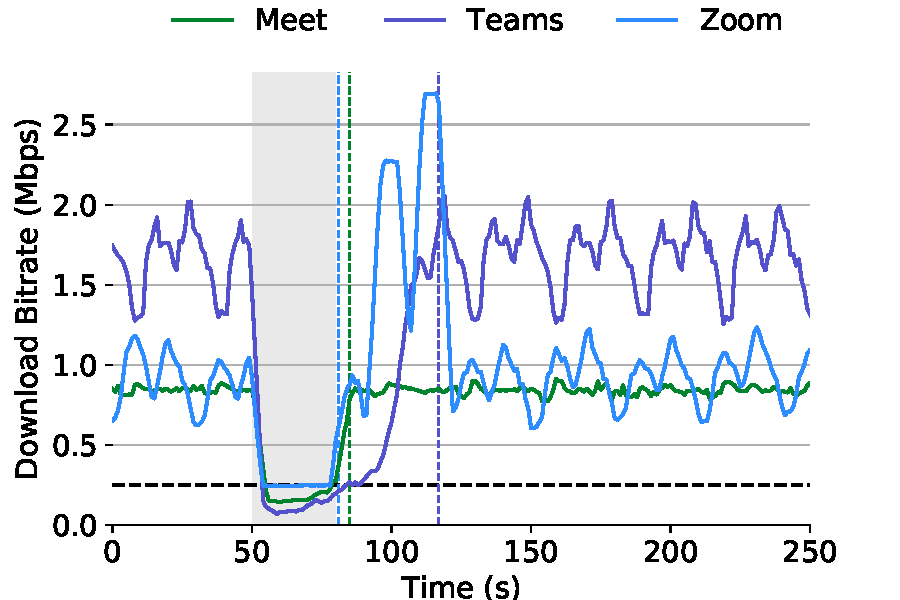
\includegraphics[width=.7\textwidth,keepaspectratio]{interrupt/Interrupt-dnld.pdf}
    \caption{Average downlink bitrate over time. Grey region indicates period where downlink capacity is constrained to 0.25 Mbps. Vertical dotted lines indicate when the dowlink bitrate has returned to the average.}
    \label{fig:ts-dnld}
\end{subfigure}
\begin{subfigure}[t]{.5\textwidth}
  \centering
    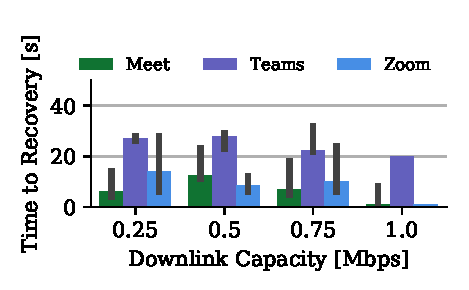
\includegraphics[width=.7\textwidth,keepaspectratio]{figures/interrupt/TTR-dnld.pdf}
    \caption{Time to recover.}
    \label{fig:TTR_dnld}
\end{subfigure}
\caption{Response to a 30s drop in available downlink capacity.}
\label{fig:interrupt-dnld}
\end{figure}

\subsection{Downstream Disruptions}

Figure~\ref{fig:TTR_dnld} shows that Teams recovers more slowly than Meet and
Zoom, always taking at least 20 seconds longer to return to the average rate,
regardless of the magnitude of the interruption. Furthermore, Meet and Zoom
recover much more quickly in this case compared to uplink interruptions. This
can be explained by the way each VCA sends video. For all three VCAs, the
clients communicate through an intermediary server. Thus, the recovery times
depend on the congestion control behavior at the server, as well. 

As mentioned in Section~\ref{sec:static}, Meet uses an encoding technique
called simulcast, where the client encodes the same video at different quality
levels and sends the encoded videos to an intermediate server. The server then
sends the appropriate version based on the perceived downlink capacity at the
receiver. The server can quickly switch between versions based on downstream
capacity to the receiver. This quick recovery is shown in
Figure~\ref{fig:interrupt-dnld}: Meet returns to its average rate in under ten
seconds, regardless the severity of the interruption.

Similarly, Zoom uses \textit{scalable video coding} when transmitting
video~\cite{zoom_encoding}. Instead of sending several versions of varying
quality, Zoom sends many hierarchical encoding layers that, when combined,
produce a high quality video. This allows C2 to continue sending uninterrupted
even when C1's downlink capacity decreases. The server can then recover faster
by sending additional layers once the network conditions improve.  

\begin{figure}[t]
    \centering
    \includegraphics[width=0.35\textwidth,keepaspectratio]{../figures/interrupt/Interrupt-sender.pdf}
    \caption{Client 2 (C2) uplink bitrate. Grey region indicates when C1's downlink capacity is reduced to 0.25 Mbps}
    \label{fig:interrupt-sender}
\end{figure}

\begin{figure}[]
   \centering
    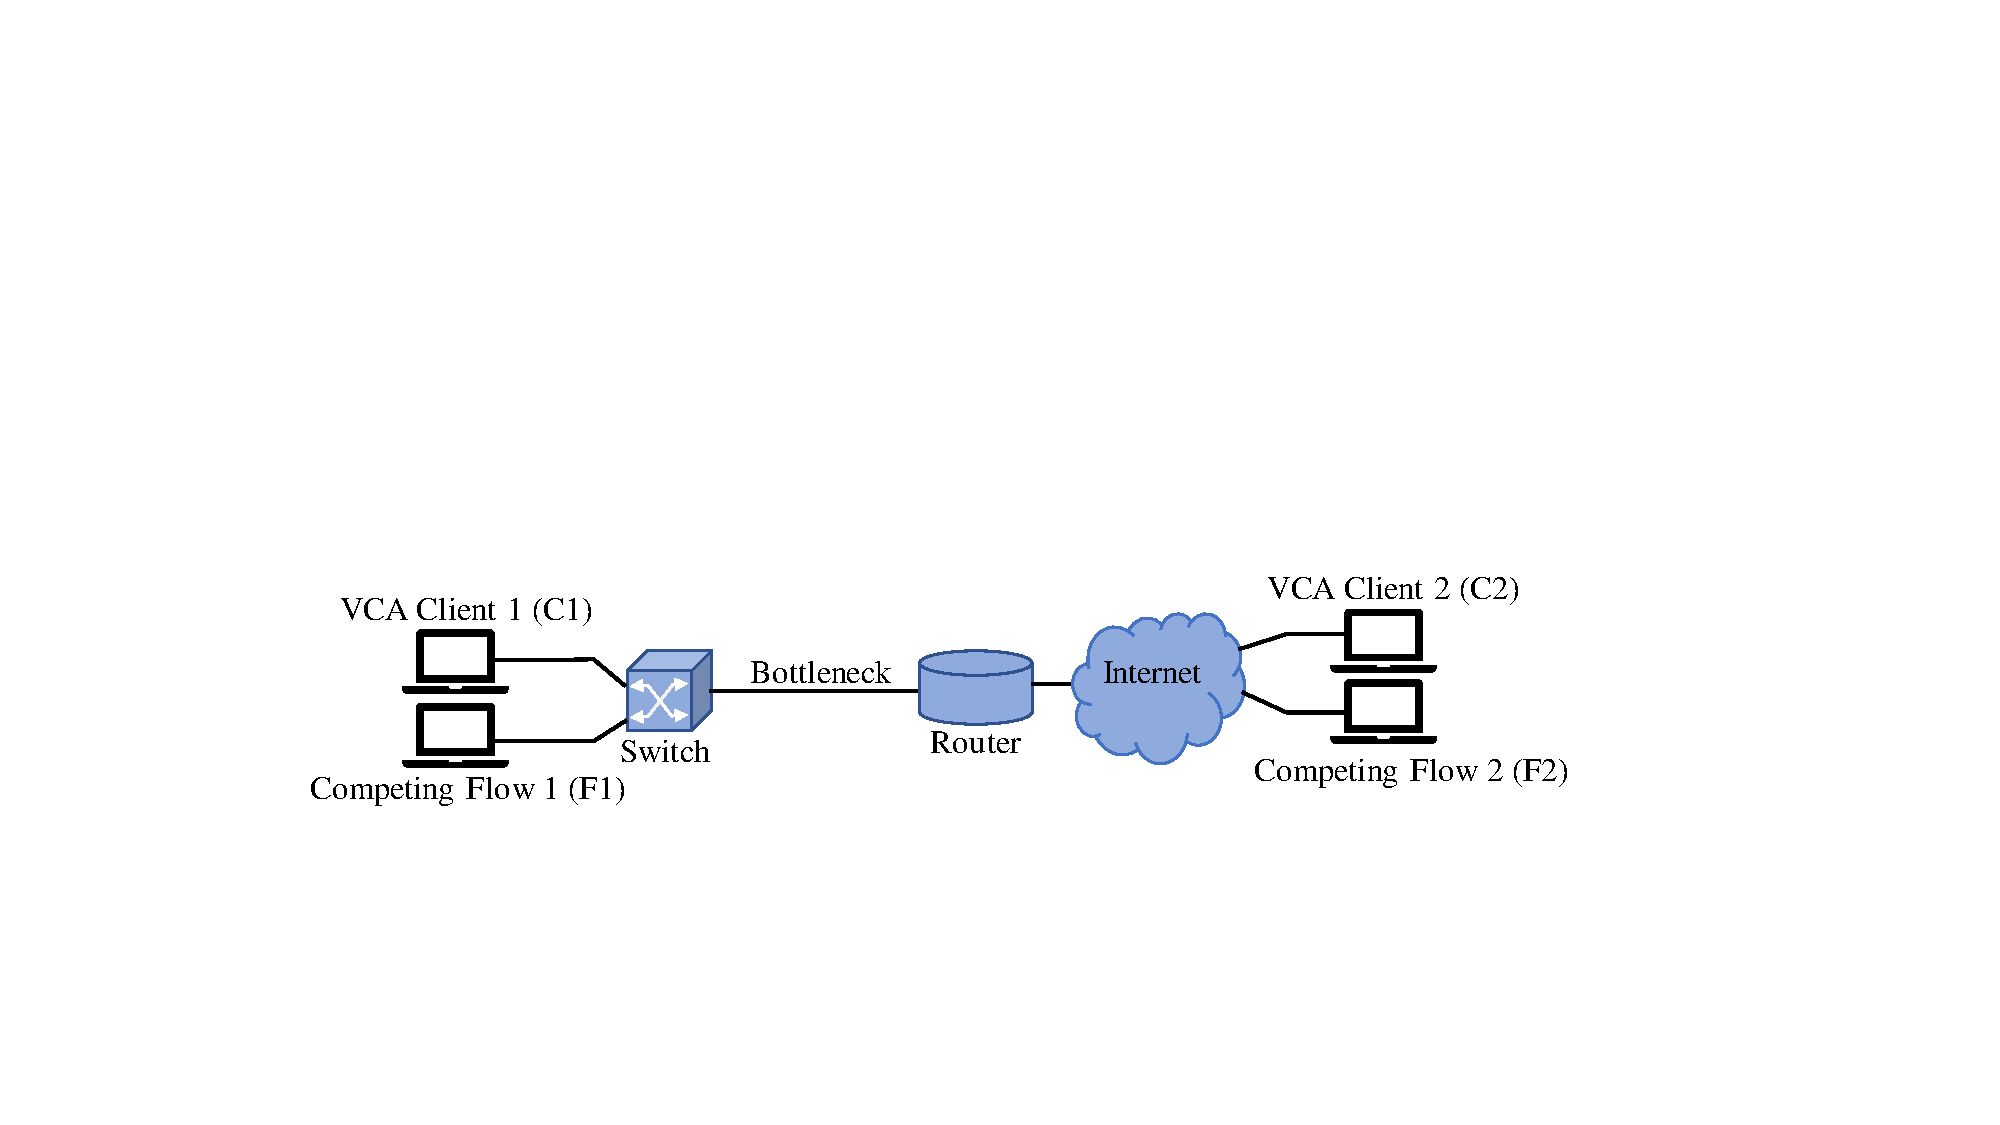
\includegraphics[width=0.5\textwidth,keepaspectratio]{methodology/competition-setup.pdf}
    \caption{Setup for competition experiments.}
    \label{fig:competition-setup}
\end{figure}


\begin{figure*}[t!]
    \centering
    \begin{subfigure}[t]{.33\textwidth}
        \centering
        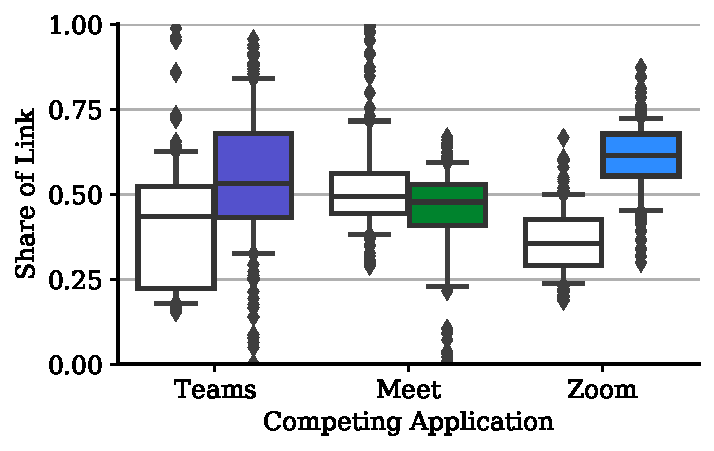
\includegraphics[width=1\textwidth]{figures/comp/box_plot_meet_ul_0.5_all.pdf}
        \caption{Meet}
        \label{fig:meet_ul_box}
    \end{subfigure}\hfill
    \begin{subfigure}[t]{.33\textwidth}
        \centering
        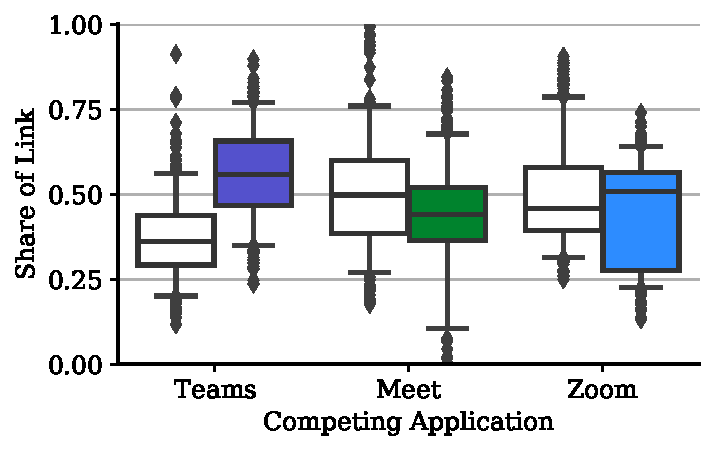
\includegraphics[width=1\textwidth]{figures/comp/box_plot_teams_ul_0.5_all.pdf}
        \caption{Teams}
        \label{subfig:teams_ul_box}
    \end{subfigure}
    \begin{subfigure}[t]{.33\textwidth}
        \centering
        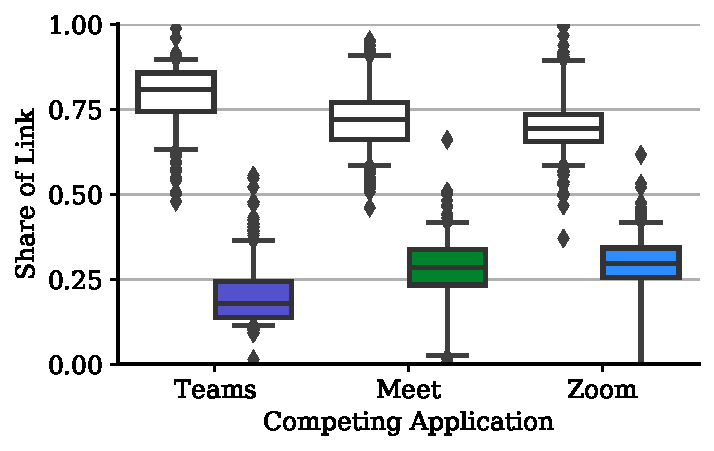
\includegraphics[width=1\textwidth]{figures/comp/box_plot_zoom_ul_0.5_all.pdf}
        \caption{Zoom}
        \label{fig:zoom_ul_box}
    \end{subfigure}
    \caption{Upstream bitrate of applications in competition with each VCA, with a symmetric link capacity of 0.5~Mbps.}
    \label{fig:boxplot-upld}
\end{figure*}

While the intermediary server for Zoom and Meet performs congestion control,
in the case of Teams, this intermediary server acts only as a relay. During a
Teams call, C2 will recognize C1 has limited downstream capacity and adjust
its sending behavior, sending at only the bitrate it knows C1 can receive.
Once C1 has more available bandwidth, C2 must discover this: it must first
probe the connection before returning to its average sending rate.
Figure~\ref{fig:interrupt-sender} illustrates how C2's sending rate does not
change during a Meet call, but drops below the shaping threshold during a
Teams call, leading to the slow recovery.

Zoom's downstream and upstream bitrates remain at the level of available
capacity during the disruption; on the other hand, Meet and Teams suffer more
serious degradation. Zoom's efficient network utilization and response to
disruption may be due to its encoding mechanisms, wherein it can more
effectively control the encoding parameters (i.e., SVC-encoded layers, FPS,
resolution etc.) to match the target bitrate.  

\begin{mdframed}[roundcorner=5pt, backgroundcolor=black!10] \noindent
    \textbf{Takeaways}: Modern VCAs are slow to recover from reductions in upstream 
    capacity, with all three requiring more than 25 seconds to recover from severe
    interruptions to 0.25 Mbps. Only Teams is consistently slow to recover
    from disruptions to downstream capacity, even showing degradation in
    response to more moderate capacity reductions (e.g., to 1 Mbps).
    This result can be attributed to each VCA's media sending mechanism and how
    congestion control is implemented at the intermediate server for each VCA. 
\end{mdframed}


